\documentclass{article}

% if you need to pass options to natbib, use, e.g.:
% \PassOptionsToPackage{numbers, compress}{natbib}
% before loading nips_2017
%
% to avoid loading the natbib package, add option nonatbib:
% \usepackage[nonatbib]{nips_2017}


% to compile a camera-ready version, add the [final] option, e.g.:
% \usepackage[final]{nips_2017}

\usepackage[final]{nips_2018}

\usepackage[utf8]{inputenc} % allow utf-8 input
\usepackage[T1]{fontenc}    % use 8-bit T1 fonts
\usepackage{hyperref}       % hyperlinks
\usepackage{url}            % simple URL typesetting
\usepackage{booktabs}       % professional-quality tables
\usepackage{amsfonts}       % blackboard math symbols
\usepackage{nicefrac}       % compact symbols for 1/2, etc.
\usepackage{microtype}      % microtypography
\usepackage{graphicx}

\title{Kaggle Competition : TMDB Box Office Prediction with Deep Neural Network}

\author{%
	Cheng Chi Fung (12219691)\\
	\texttt{cfchengac@connect.ust.hk} \\
}

\begin{document}

\maketitle

\begin{abstract}
In this project, we try to applying deep neural network to tackle the TMDB Box Office Prediction Compeition ( \url{https://www.kaggle.com/c/tmdb-box-office-prediction/data}), a box office revenue prediction competition based on the metadata of past films from The Movie Database (TMDB). The architecture of our deep neural network is mainly composed by attention-based bi-LSTM, Resnet and feedforward network with attention and it is trained by the movie data after feature enginerring that achieves a test set minimum MST Loss of 0.5991 and obtain the score 2.66035 on kaggle platform.
\end{abstract}

\section{Introduction}

\subsection{Box Office Prediction}
Film industry is booming, the revunues are growing, so we have a lot of data about films. What we want to see is if we can use the latest advances in artificial intelligence to accurately predict film revenues in order to make some changes in movies to increase their revenues even further.

\subsection{Box Office with Deep Neural Network} 

Moreover, we find that most of the participants in this kaggle compeition using some popular machine learning model like xgboost or lightgbm to solve the problem and achieve a very good results (from kaggle discussion and kernel) and only a few of the participants neural network. Therefore, in the project, we also want to see the performance of applying deep neural network in this problem.

\subsection{Problem Statement}

In this probject, we are going to implement a deep neural network model by using the only data source, the dataset given in the competition to predict the box office revenue. The implemented model would be allowed to takes moive's features, included its categorical, text, image and numerical features. And the model would then outputs the predicted box office revenue.

\section{Dataset}

The dataset used in this project is the movie dataset given in this kaggle compeition, which is a dataset consisting of 7,398 past films metadata  collected from The Movie Database (TMDB). Moreover, this dataset has been further seperated into training set and test set which consists of 3,000 films and 4,398 films metadata respectively. The data point in the dataset includes the films's cast, crew, plot keywords, budget, posters, release dates, languages, production companies, and countries etc. The full list of the features in the metadata are as follow.

\begin{table}[htb]
	\caption{dataset columns}
	\label{sample-table}
	\centering
	\begin{tabular}{l}
		\toprule
		\cmidrule{1-1}
		Columns  \\
		\midrule
		belongs\_to\_collection \\
		budget  \\
		genres \\
		homepage  \\
		imdb\_id  \\
		original\_language \\
		original\_title	  \\
		overview  \\
		popularity  \\
		poster\_path  \\
		popularity  \\
		production\_companies \\
		production\_countries \\
		release\_date \\
		runtime \\
		spoken\_languages \\
		status \\
		tagline \\
		title \\
		Keywords \\
		cast \\
		crew \\
		revenue \textbf{(Only in training set)}\\
		\midrule
	\end{tabular}
\end{table}

\pagebreak

\subsection{Exploratory Data Analysis}
Before the data preprocessing, some analysis has been performed on the training sets to summarize their main characteristics.


\subsubsection{Number of Missing Values}
\begin{figure}[h]
  \centering
  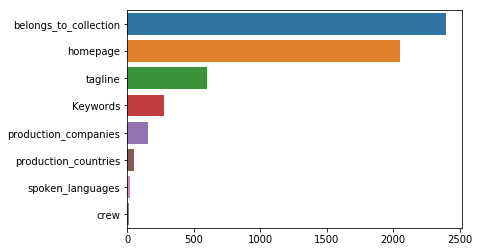
\includegraphics[scale=0.7]{collections.png}
  \caption{Number of missing values in each columns}
\end{figure}

belongs\_to\_collections and home\_page contain so many missing value, it is better to drop it or extract some new feature from them.

\subsubsection{Tag lines}
\begin{figure}[h]
  \centering
  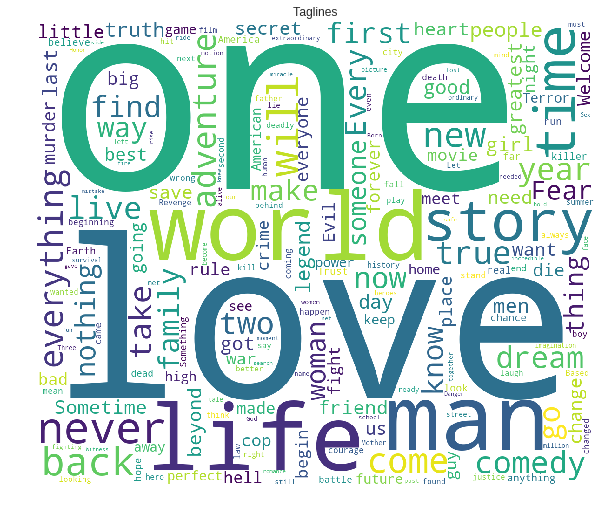
\includegraphics[scale=0.5]{taglines.png}
  \caption{taglines word cloud}
\end{figure}

Most of the films in the training set are related to love, story, world and life.
\pagebreak

\subsubsection{Production Countries}
\begin{figure}[h]
  \centering
  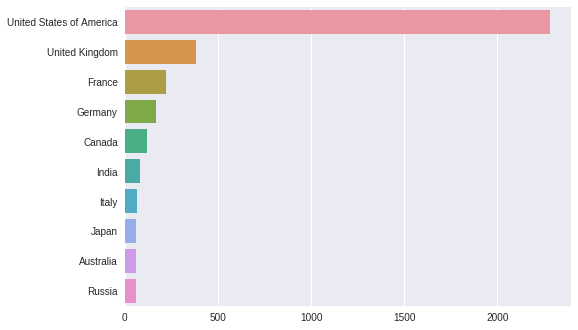
\includegraphics[scale=0.7]{production_com.png}
  \caption{top production countries}
\end{figure}

Most of the films are produced in USA, UK and France. For the film of that come from the countries which only produce small number of films such as Russia. It may be difficult to predict their revenues using our model.
\pagebreak

\subsubsection{Spoken Languages}
\begin{figure}[h]
  \centering
  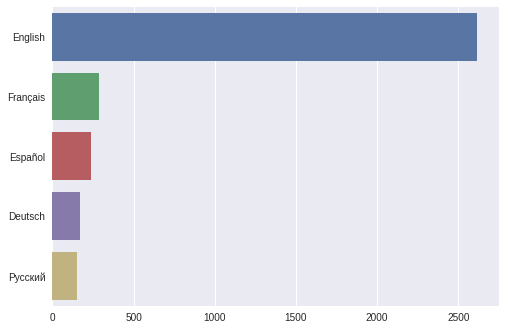
\includegraphics[scale=0.7]{lang.png}
  \caption{top production countries}
\end{figure}

Most of the films has the spoken languages of English, France, Espafnol. It is interested that Russian get the top five in spoken language but not appear in the top five of production countries.

\subsubsection{Genres}
\begin{figure}[h]
  \centering
  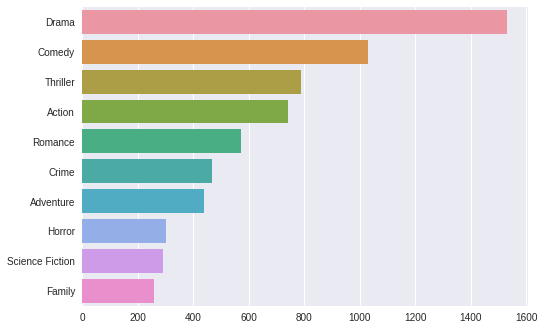
\includegraphics[scale=0.7]{genres.png}
  \caption{top genres}
\end{figure}

Drama is the most common. Comedy and Drama film conquer nearly half of the training set.

\pagebreak

\subsubsection{Revenues}
\begin{figure}[h]
  \centering
  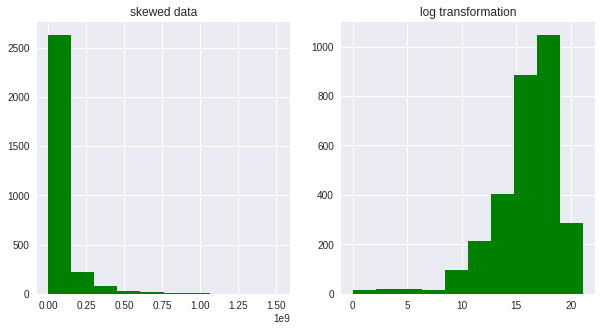
\includegraphics[scale=0.7]{revenue.png}
  \caption{Revenue}
\end{figure}

The revenue is left skewed. Log tranform may need to apply to make it normal disturbuted.

\subsubsection{Budgets}
\begin{figure}[h]
  \centering
  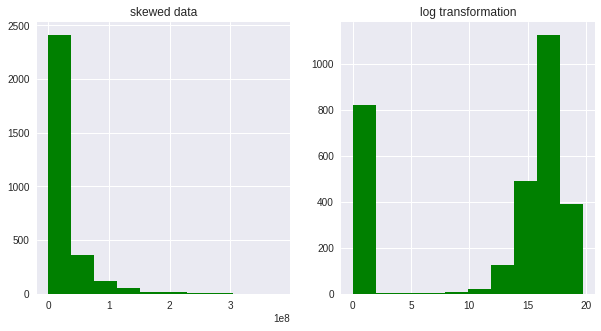
\includegraphics[scale=0.7]{budget.png}
  \caption{Budgets}
\end{figure}

A interested effect in budgets is that a larget number of films has zero budgets. It may be a problem if we use budget as the feature input.
In addition, the budget is left skewed. Log tranform may need to apply to make it normal disturbuted.

\pagebreak


\subsubsection{Popularity}
\begin{figure}[h]
  \centering
  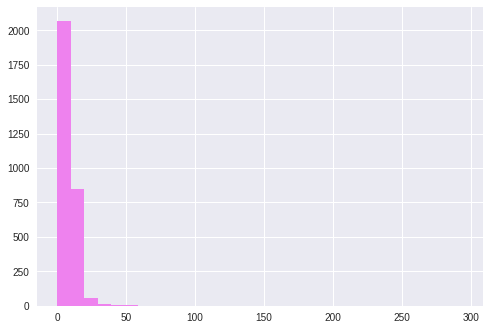
\includegraphics[scale=0.7]{popularity.png}
  \caption{Popularity}
\end{figure}

The popularity is left skewed. Log tranform may need to apply to make it normal disturbuted.

\subsubsection{Budgets Mean by Year}
\begin{figure}[h]
  \centering
  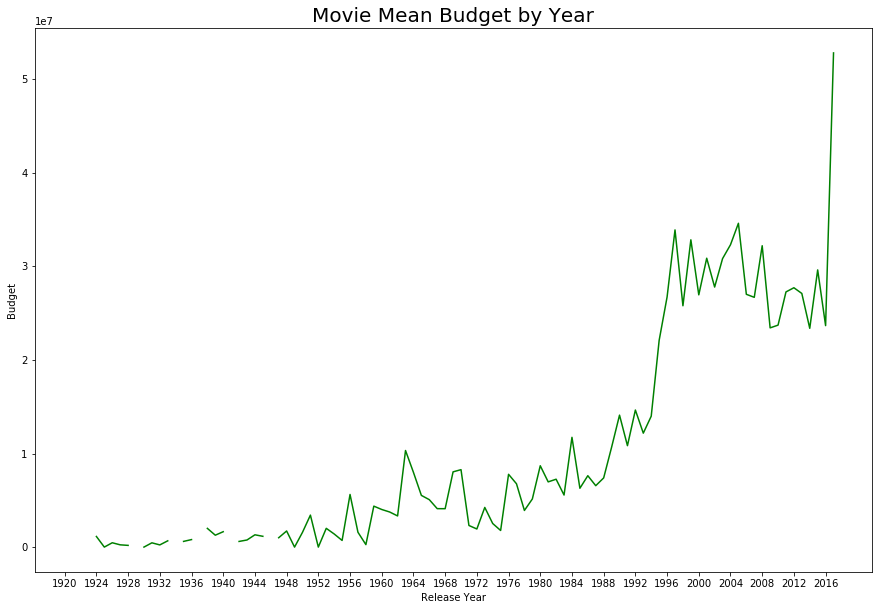
\includegraphics[scale=0.4]{mean_budget.png}
  \caption{Popularity}
\end{figure}

We can see the budget is increasing each year. This may be because of inflation.


\subsection{Data Preprocessing and Feature Enginerring}

Before the data are feeded into the neural network, some feature enginerring and data preprocessing are performed to enhance the training performance. And it is mainly composed by four parts (Feature Selection, Data Cleaning, Encoding and Feature transformation)


\subsubsection{Feature Selection}

	In feature selection part, some new features are extracted from the metadata and some not meaningful features are dropped. 
	
The following are the new features we have extracted.
	
	\begin{table}[htb]
	\caption{new features extracted}
	\label{sample-table}
	\centering
	\begin{tabular}{ll}
		\toprule
		\cmidrule{1-2}
		New Features &  Extracted from Feature \\
		\midrule
		release\_day & release\_date \\
		release\_month & release\_date \\
		release\_year & release\_date \\
		production\_countries\_count & production\_countries \\
		production\_companies\_count & production\_companies \\
		cast\_count & cast \\
		crew\_count & crew \\
		num\_Keywords & Keywords \\
		inflationBudget & budgets \\
		
	\end{tabular}
\end{table}
	
	For the release\_date, since the original format of release\_date is difficult to be input into the neural network. Therefore, three new features, release\_year, release\_month and release\_day will be extracted from release\_date.
	
	For the production\_countries\_count, production\_companies\_count, cast\_count, crew\_count and num\_Keywords, some experiements from (\url{https://www.kaggle.com/zero92/tmdb-prediction}) has found out that these new features can boost the performance. And in fact, these extra features can help us to ease down the difficulty of training the neural network for prediction.
	
	For inflationBudget, since the original budgets has not take consideration of the effect of inflation. Therefore, we base on the original budget with Inflation simple formula to caculate the budget of the film after inflation.
	
The following are the features we dropped.
	\begin{table}[htb]
	\caption{dropped features}
	\label{sample-table}
	\centering
	\begin{tabular}{ll}
		\toprule
		\cmidrule{1-2}
		Dropped Features & Drop Reason \\
		\midrule
		homepage & url is difficult to use\\
		status & constant feature \\  
		original\_language & almost same as the spoken\_language column \\
		original\_title & almost almost same as the title column \\
		imdb\_id\ & unique value \\
	\end{tabular}
\end{table}

After performing the feature selection, the following features  are used in the prediction part and we can categories them into four types, namely catatogical, numerical, text and image.

\begin{table}[htb]
	\caption{selected features after feature selection}
	\label{sample-table}
	\centering
	\begin{tabular}{ll}
		\toprule
		\cmidrule{1-2}
		Features &  Types \\
		\midrule
		belongs\_to\_collection & categorical \\
		budget & numerical \\
		genres & categorical \\
		overview & text \\
		popularity & numerical \\
		poster & image  \\
		popularity & numerical  \\
		production\_companies  & categorical \\
		production\_countries   & categorical\\
		release\_day  & numerical \\
		release\_month  & numerical \\
		release\_year   & numerical\\
		runtime  & numerical \\
		spoken\_languages & categorical\\
		tagline & text \\
		title & text \\
		Keywords & text \\
		cast & categorical\\
		crew & categorical\\
		revenue  & numerical \\
		production\_countries\_count & numerical\\
		production\_companies\_count & numerical\\
		cast\_count & numerical\\
		crew\_count & numerical\\
		num\_Keywords & numerical\\
		inflationBudget & numerical\\
		\midrule
	\end{tabular}
\end{table}



		

\pagebreak

\subsubsection{Data Cleaning}
	In data cleaning part, the features with missing value are filled and transfer into the easy processable format. In addition, the text features are cleaned with serveral procedures.
	
	For all the columns having the dictionary format in the metadata (belongs\_to\_collection, genres, production\_companies, production\_coutries, spoken\_languages, Keywords, cast, crew), we extract the value with the key "name" and give up all other things such as id in the dict . For the other columns, we keep them as the original forms as in the meta data.
	
	For all the catagorical features, we fill all the missing value by "!". Moreover, for the scalar columns, we fill the missing value by their median since it is more resistant to  outlier.
	
	Moreover, for the data cleaning of the text features, we first turn all the unicode string into \textbf{ASCII} and \textbf{lower case}. Then, we \textbf{expand the contradiction} and \textbf{remove all the characters except (A-Za-z0-9,.!?;)}.
	
\subsubsection{Data Encoding}
	In encoding part, all the catagorical feature are encoded into one hot representation.

\subsubsection{Feature Transformation}
In feature transformation part, the scalar features are transformed into the disturbution that are easily trained by neural network. The transofmations of the scalar columns are shown below.

\begin{table}[htb]
	\caption{feature transformation}
	\label{sample-table}
	\centering
	\begin{tabular}{ll}
		\toprule
		\cmidrule{1-2}
		Features &  Transformations \\
		\midrule
		revenues & log transform, standardize \\
		budget & log transform, standardize \\
		popularity & log transform, standardize \\
		runtime & log transform, standardize \\
		release\_day & cyclic transform, standardize \\
		release\_month & cyclic transform, standardize \\
		release\_year & standardize \\
	\end{tabular}
\end{table}

For log transform, it refers to applying log to transform the feature which turn the skewed data into normal like disbutrubtion. For cyclic transform, we take a reference from \url{(https://ianlondon.github.io/blog/encoding-cyclical-features-24hour-time/)}. It used is to encode the cyclical continuous features into encoding with cyclical nature. For standardize, it transforms the feature into mean = 0 and variance = 1.

For image features, they are transformed into grey scale with normalization.

\pagebreak



\section{Deep Neural Network}

\subsection{Architecture}
In the project, we try to apply deep neural network to predict the box office revenues. The archiecture of the deep neural network is composed by four different encoders to encode different types of input features and the main net. 

\begin{figure}[h]
  \centering
  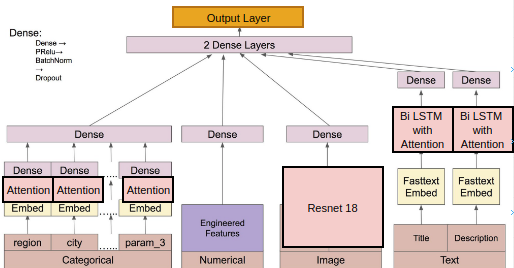
\includegraphics[scale=1]{map.png}
  \caption{The archiecture of the our deep neural network}
\end{figure}

\subsubsection{Categorical Encoder}

The categorical encoder in our network is to encode all catagorical features. It is composed by an embedding layer to embbed the feature inputs, an additive attention layer to handle the features that can have \textbf{multiple values} such as genres. (A film can have multiple genres), and two dense layers to embed all categorical features into a feature vector.

\pagebreak

\begin{figure}[h]
  \centering
  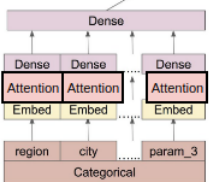
\includegraphics[scale=1]{cat.png}
  \caption{Categorical Encoder}
\end{figure}


\subsubsection{Numerical Encoder}

The numerical encoder in our network is to encode the numerical features. It is composed by a dense layer to embed all the numerical feature in to a feature vector.

\begin{figure}[h]
  \centering
  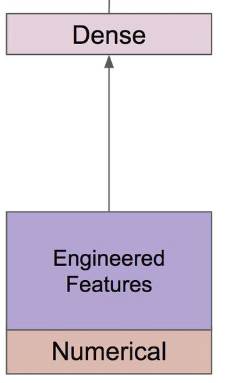
\includegraphics[scale=0.5]{numerical.png}
  \caption{Numerical Encoder}
\end{figure}

\subsubsection{Text Encoder}


The text encoder in our network is to encode the text features. It is composed by a word2Vector  embedding layer, an Attention Based Bi-LSTM layer and a dense layer to embbed the text feature into a context vector.

For the word embedding layer, it has been pretrained with \textbf{Google News corpus} (3 billion running words) word vector model. (Google News Corpus: \url{https://github.com/mmihaltz/word2vec-GoogleNews-vectors)}. And since the dimension of the embedding matrix is enormously big which cause some memory error during training, we have limited to only use ten thousands of vocabs. All above process can be easily done through a python libarary named \textbf{gensim}.

For Attention Based Bi-LSTM, the archiecture of is same as the paper \textbf{Attention-Based Bidirectional Long Short-Term Memory Networks for Relation Classification} (\url{https://www.aclweb.org/anthology/P16-2034}) which use two LSTM in reverse direction and using addition attention for caculating the final context vector from each of the hidden states in LSTMs.

\begin{figure}[h]
  \centering
  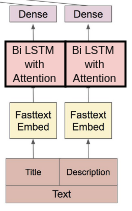
\includegraphics[scale=1]{rnn.png}
  \caption{Text Encoder}
\end{figure}

\subsubsection{Image Encoder}

The image encoder in our network is to encode the image feature. It is composed by a pretrained \textbf{18 layers ResNet} and a dense layer to embed image feature in to a feature vector. 

The pretained resnet can be easily done through a python libarary named \textbf{torchvision.models}

\begin{figure}[h]
  \centering
  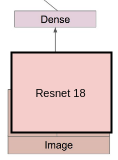
\includegraphics[scale=1]{cnn.png}
  \caption{Image Encoder}
\end{figure}

\subsubsection{Main Net}

The main net is used to concatenate all the feature vectors from different encoders and predict the final results. It is compose by two dense layers and a output layer with a hidden unit.

\pagebreak

\begin{figure}[h]
  \centering
  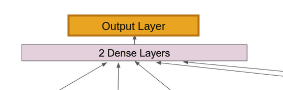
\includegraphics[scale=1]{main.png}
  \caption{Main Net}
\end{figure}

\subsubsection{Dense Layer settings}

The dense layer setting in our network are as follow. Except the last dense layer and the output layer, all dense layers in the network is followed by a \textbf{Randomized Leaky ReLU (RReLU)} , a batch noralization layer and a dropout layer

\begin{table}[htb]
	\caption{Dense Layer Setting}
	\label{sample-table}
	\centering
	\begin{tabular}{llll}
		\toprule
		\cmidrule{1-4}
		Setting & Other dense layers  & Last dense Layer in Main Net & Output Layer \\
		\midrule
		Dense & * & * & *\\
		RReLu & * & *\\
		BatchNorm & * &\\
		Dropout & * &\\
		\midrule
	\end{tabular}
\end{table}



\section{Experimental Setting}

For the experiment, we have further splitted the training set into training set and validation set with the ratio 8:2. We first traing out model using the training set and perform the hyperparameters performance evluation using the validation set with different hyperparameters. After hyperparameters tuning, we train the model with the best hyperparameter obtained and test the model on the test set. Moreover, the training is to be early stopped when the validation MSE Loss has decreased for specified number of epochs.


\subsection{Computational Environment}

All the experiment conducted in this project using the following computational environment. 
\begin{table}[htb]
	\caption{Computational Environment}
	\label{sample-table}
	\centering
	\begin{tabular}{ll}
		\toprule
		\cmidrule{1-2}
		Computational Settings & -- \\
		\midrule
		CPU & AMD Ryzen 2700x \\
		GPU & RTX2080Ti \\
		RAM & 32GB \\
		OS & Ubututu 16.04 \\
		Python Version & 3.5 \\
		Deep Learning Libarary & Pytorch \\
		\midrule
	\end{tabular}
\end{table}
\subsection{Hyperparameters Tuning}
For the hyperparameters tuning, we perform grid search to find the best hyper-parameters (drop out rate, learning rate and the the number of hidden units in the last dense layer of main net)

\subsubsection{Hyperparameters Tuning Environments}
For the hyperparameters tuning, the following training environment are used. 

\pagebreak

\begin{table}[htb]
	\caption{Tuning Environment}
	\label{sample-table}
	\centering
	\begin{tabular}{ll}
		\toprule
		\cmidrule{1-2}
		Tune Settings & -- \\
		\midrule
		Epoch & 100 \\
		Optimizer & Adam \\
		Batch Size & 32 \\
		Early Stopping & 30 \\
		\midrule
	\end{tabular}
\end{table}


\subsubsection{Hyperparameters Tuning Results}


\begin{table}[htb]
	\caption{Hyperparameter tuning results}
	\label{sample-table}
	\centering
	\begin{tabular}{llll}
		\toprule
		\cmidrule{1-4}
		Learning Rate & Dropout rate & Number of hidden units in Last Layer & Best Validation MSE Loss\\
		\midrule
		0.1 & 0.25  & 200 & 0.7231  \\
		0.05 & 0.25  & 200 & 0.7532 \\
		0.01 & 0.25  & 200 & 0.6672\\
		0.005 & 0.25  & 200 & 0.634 \\
		0.001 & 0.25  & 200 & 0.6011\\
		0.0005 & 0.25  & 200 & 0.6343 \\
		0.0001 & 0.25  & 200 & 0.6314 \\
		0.1 & 0.25  & 200 & 0.7356\\
		0.1 & 0.30  & 200 & 0.7422 \\
		0.01 & 0.35  & 200 & 0.7245 \\
		0.01 & 0.40  & 200 & 0.6035 \\
		0.01 & 0.45  & 200 & 0.6422 \\
		0.01 & 0.50  & 200 & 0.6135 \\
		0.01 & 0.30  & 200 & 0.6314\\
		0.01 & 0.30  & 300 & 0.6456\\
		0.01 & 0.30  & 500 & 0.6042\\
		0.01 & 0.30  & 1000 & 0.7324\\
		\bottomrule
	\end{tabular}
\end{table}

Best Parameters Hyperparameter obtained { learning rate : 0.001, Dropout: 0.4, Number of Hidden Unit: 500}

 
\subsection{Final Training Parameters Settings and Environment}

We use the best hyperparameters obtained from hyperparameters tuning and train the model same as the architecture above with the following parameters settings.

\begin{table}[htb]
	\caption{Training Parameters Settings}
	\label{sample-table}
	\centering
	\begin{tabular}{ll}
		\toprule
		\cmidrule{1-2}
		Parameters & -- \\
		\midrule
		Epoch & 1200 \\
		Optimizer & Adam \\
		Batch Size & 64 \\
		Early Stopping & 100 \\
		Learning Rate & 0.001 \\
		Dropout & 0.4 \\
		\midrule
	\end{tabular}
\end{table}


\section{Results and Analysis}

\subsection{Performance}
The following are the results of the final training with the specification in the last past. You can find me on the leaderboard with the name fingnn.

\begin{table}[htb]
	\caption{Score in Kaggle}
	\label{sample-table}
	\centering
	\begin{tabular}{ll}
		\toprule
		\cmidrule{1-2}
		Dataset & Best Score\\
		\midrule
		Test Set & 2.66035   \\
		\bottomrule
	\end{tabular}
\end{table}

\begin{table}[htb]
	\caption{Best MSE Loss in Validation Set}
	\label{sample-table}
	\centering
	\begin{tabular}{ll}
		\toprule
		\cmidrule{1-2}
		Dataset & Best MSE Loss\\
		\midrule
		Validation Set & 0.5991   \\
		\bottomrule
	\end{tabular}
\end{table}

\pagebreak

\begin{table}[htb]
	\caption{Time Used for the experiments}
	\label{sample-table}
	\centering
	\begin{tabular}{ll}
		\toprule
		\cmidrule{1-2}
		Module & Wall time \\
		\midrule
		Parameter Tuning & 7.12 hours \\
		Final Training & 1.1 hours \\
		\midrule
	\end{tabular}
\end{table}





\subsection{Learning Curve}
The below are the loss curve trained with best hyper-params. The blue curve is the validation MSE Loss. The orange curve are the training MSE Loss Curve.

\begin{figure}[h]
  \centering
  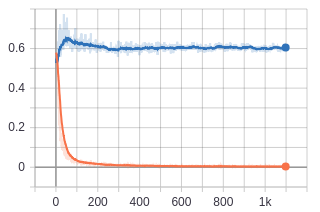
\includegraphics[scale=1]{learning_curve.png}
  \caption{MSE Loss Curve}
\end{figure}

From the results, we can see although we have apply dropout layer in the neural network but, it is still fail to lower the validation MSE Loss too much. On the other hand, for the training MSE loss, it is able to converge to minma. Therefore, although we got a very low training MSE Loss but still got a normal kaggle score.

\pagebreak

\subsection{Comparing the results to others kaggle participants}

Comparing the results to the model of other participants such as \url{https://www.kaggle.com/akumaldo/tmdb-prediction-eda-lgb-xgb-cat-plus-keras-nn}. We can see, in fact our model is not very bad. 

\begin{table}[htb]
	\caption{Results of other participants}
	\label{sample-table}
	\centering
	\begin{tabular}{ll}
		\toprule
		\cmidrule{1-2}
		Model & Best Validation MST Loss\\
		\midrule
		xgBoost & 2.0656   \\
		keras NN & 5.4218   \\
		\bottomrule
	\end{tabular}
\end{table}

\begin{figure}[h]
  \centering
  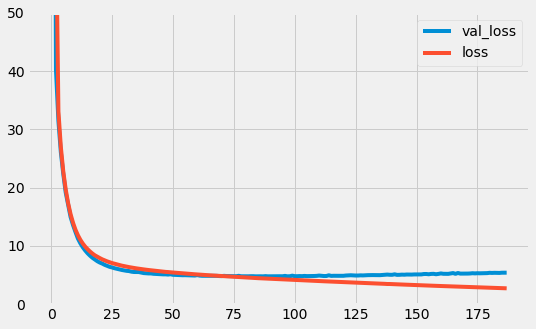
\includegraphics[scale=0.7]{other_curve.png}
  \caption{MSE Loss Curve of the Keras NN implemented by other participants}
\end{figure}

For xgBoost, we can see it done very well in regression problem. Its best validation MST loss is much lower than keras NN and our model. However, the performance for its keras NN is quite similiar to our deep neural network. Moreover, we can also see that others also face the similiar overfitting problem in training NN for solving the problem.


\subsection{Visualization of some Gradient Histogram }

In the gradient histogram, we can see the even we trained the network for 1100 epoches. The network does not have any gradient vanishing or exploding problem. All Layers contains non-zero gradients. (More Gradient Histogram can be found on running the tensorboard in logs folders.
\begin{figure}[h]
  \centering
  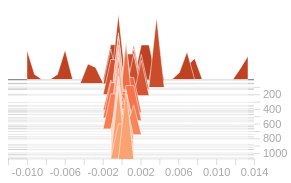
\includegraphics[scale=1]{linear_1.png}
  \caption{Gradient Histogram of Genres Layer}
\end{figure}

\begin{figure}[h]
  \centering
  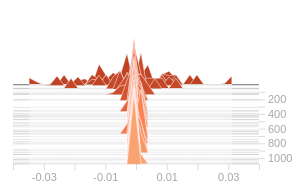
\includegraphics[scale=1]{linear_2.png}
  \caption{Gradient Histogram of Production Countries Layer}
\end{figure}

\pagebreak


\subsection{Problems}

First, it is difficult and time consuming to tune the parameters when we apply deep neural network in the regression problems. Since, unlike classification only having limited numbers of labels, for regression, the neural network need to fit so many values. Therefore, it is difficult for the neural network to converge. That is why, xgbost and lightgbm are more common and popular in kaggle competition. 

Moreover, training dataset provided by the kaggle is too small and even smaller than the test set. Therefore, it is difficult to achieve a good results without using any external data sources.

Last but not last, some data in test set having the labels that do not appear in the training set which make our model difficult to predict the data with a lot of unseen labels.

\subsection{Future Development}

To enhance the model perforance, we can replace Attension Based Bi LSTM to more advanace model like transformer.

Also, we can apply some clustering techique such as k-mean clustering to cluster the similiar data in order to fill in the missing value.

Finally, more feature enginerring can be applied to the model in order to get better platformance. We can see from the competition discussion, most of the participant perform a lot of feature enginerring works other than improving the structure of the model. 

\subsection{Conclusion}

In this project, we have explored to using deep learning to solve the regression problem in kaggle. Alrough this is difficult, it is funny.

\end{document}
